ue1:

1.Aufgabe:
\begin{equation}
	\begin{split}
		b \in \left\{ x_1 \cdot \begin{pmatrix*} 1\\ 1\\ 1 \end{pmatrix*} + x_2 \cdot \begin{pmatrix*} 1\\ -2\\ -1 \end{pmatrix*} | x_1, x_2 \in \R \right\}
	\end{split}
\end{equation}
eine möglichst \glqq gute\grqq{} Lösung könnte sinnvollerweise foglendes erfüllen:

\[
	\norm{Ax-b}^2_2 \longrightarrow min
\]

2.Aufgabe:
\captionStyle{n}{}
\bxfigure[ht]{\url{https://en.wikipedia.org/wiki/File:Projection_and_rejection.png} }
{
%	\centering
	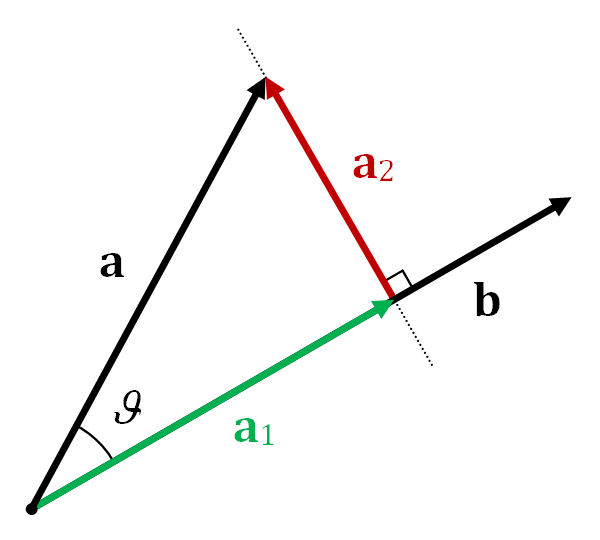
\includegraphics[scale=.3]{Projection_and_rejection.png}
}

\begin{equation}\begin{split}
	u = \begin{pmatrix*}1\\1\\1\end{pmatrix*}\quad;\quad
	v = \begin{pmatrix*}0\\2\\1\end{pmatrix*}\\
	v = v_{\bot} + v_{\parallel}\\\\
\end{split}\end{equation}
\begin{equation}\begin{split}
	<v; u>
	&= <v_{\bot} + v_{\parallel}; u>\\
	&= <v_{\bot}; u> + <v_{\parallel}; u>\\
	&= \cancelto{0}{<v_{\bot}; u>} \quad + <v_{\parallel}; u>\\
	&= <v_{\parallel}; u>\\
\end{split}\end{equation}
